% Exemplo para incluir futuramente em um capitulo de metodologia/desenvolvimento.
% Caminhos relativos a Documentacao/Doc/doc_latex, pasta de monografia.tex.
% Requer graphicx e o comando \fonte da classe abntex2 usada pelo modelo.
% Este arquivo NAO e incluido automaticamente no TCC.

\begin{figure}[htbp]
    \centering
    \caption{Arquitetura em blocos do software implementado no Raspberry Pi}
    \label{fig:arquitetura-software-rpi}
    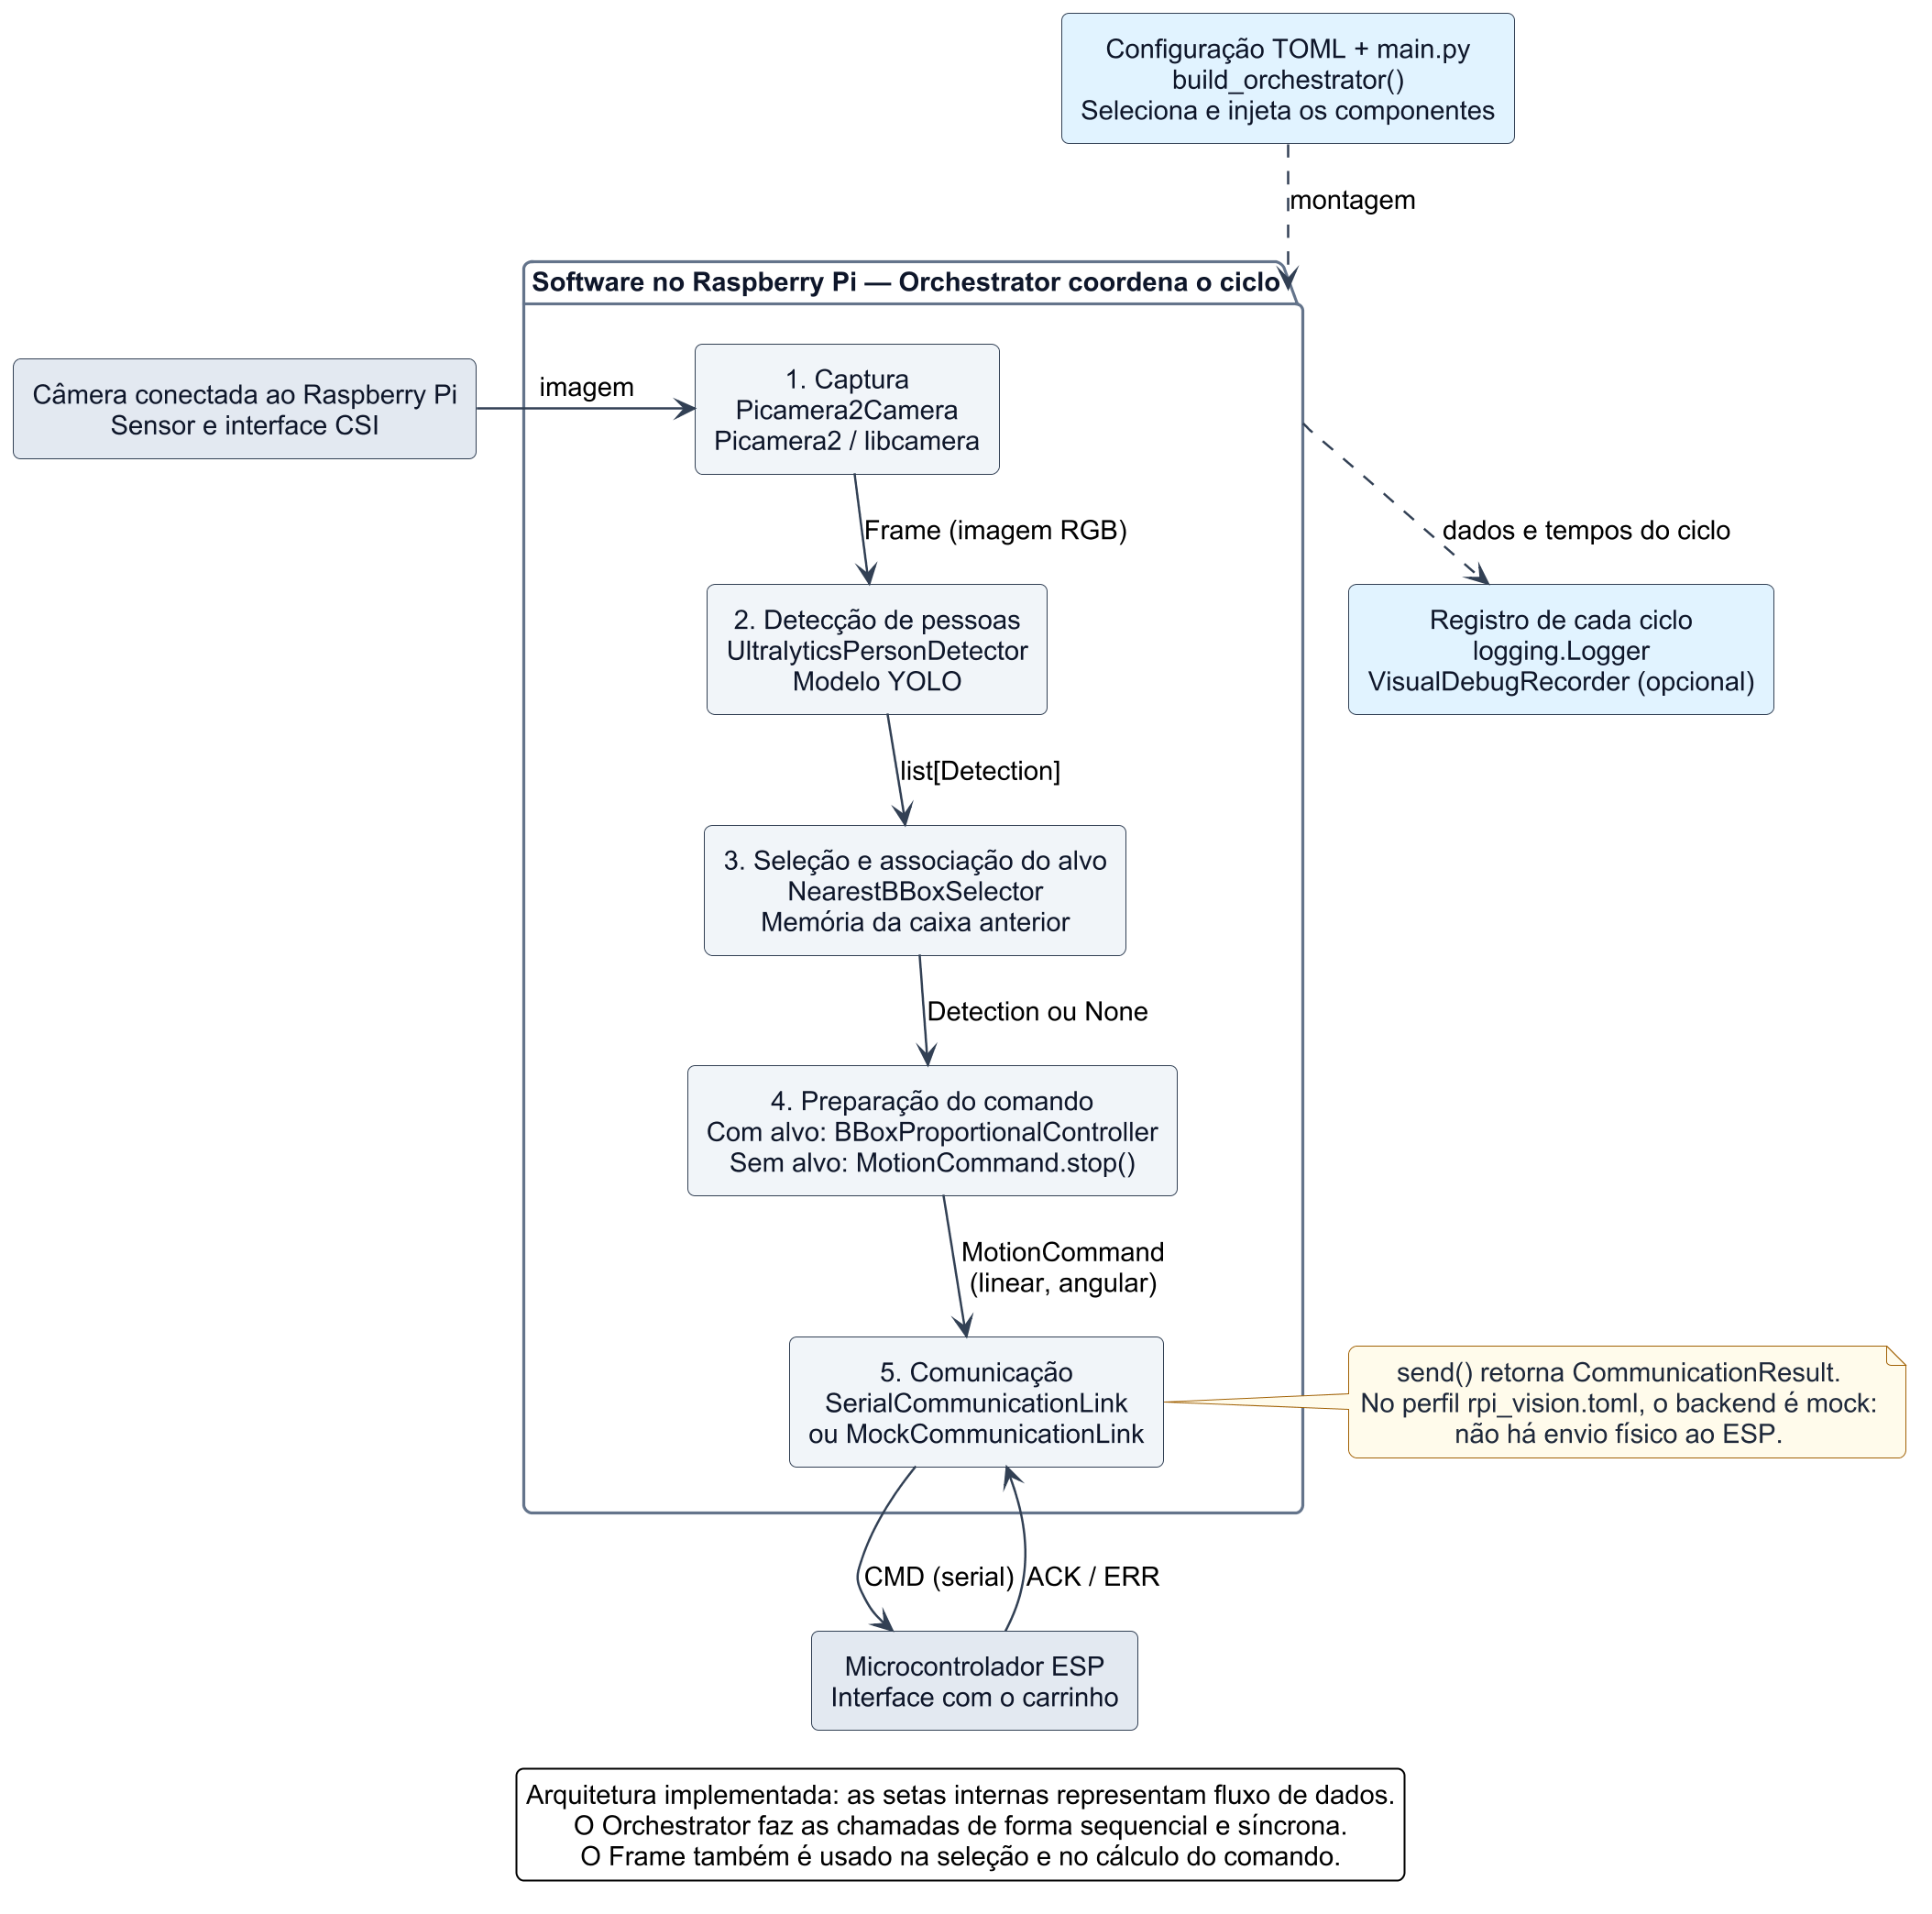
\includegraphics[width=\linewidth,height=0.78\textheight,keepaspectratio]{../../diagramas/software_rpi/renderizados/arquitetura_blocos.png}
    \fonte{Elaboração própria.}
\end{figure}

\begin{figure}[htbp]
    \centering
    \caption{Diagrama de estados proposto para o seguimento e a busca do alvo por rotação}
    \label{fig:estados-software-rpi-previsto}
    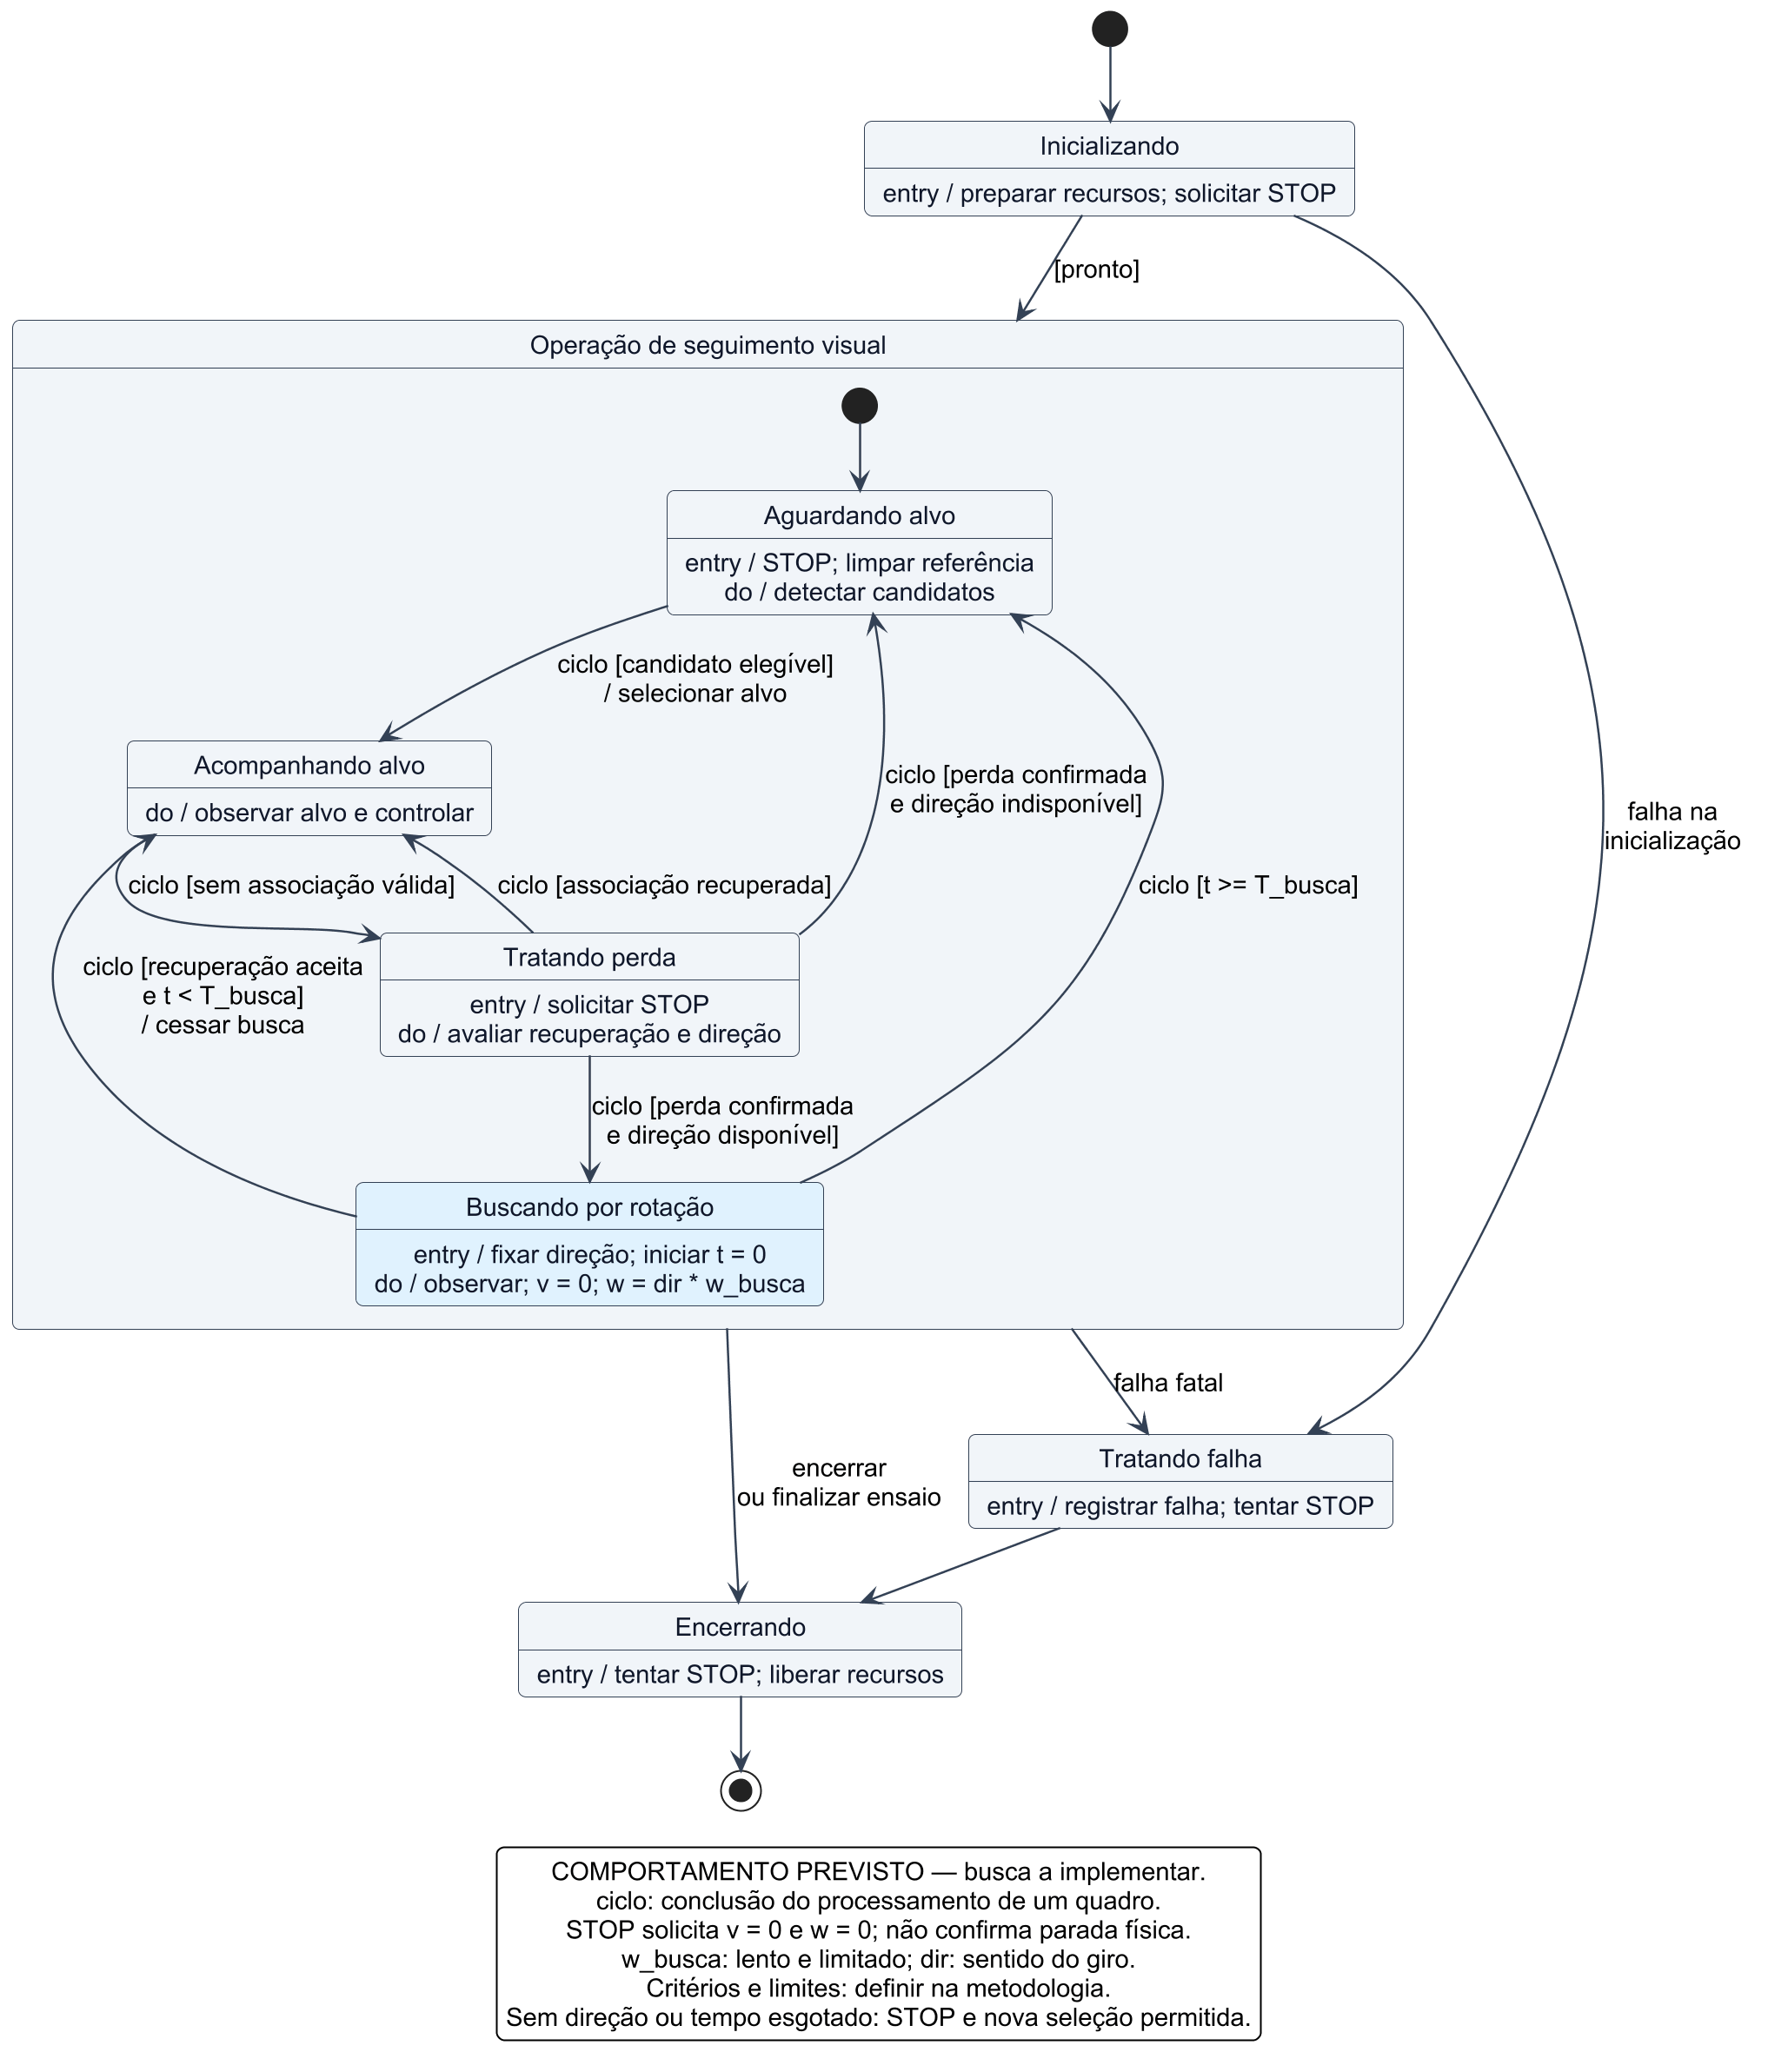
\includegraphics[width=\linewidth,height=0.78\textheight,keepaspectratio]{../../diagramas/software_rpi/renderizados/estados_rpi_previsto.png}
    \fonte{Elaboração própria.}
\end{figure}

% Exemplos de referencias no texto:
% A Figura~\ref{fig:arquitetura-software-rpi} apresenta os modulos do software.
% O comportamento proposto e representado na Figura~\ref{fig:estados-software-rpi-previsto}.
% Conferir a legibilidade no PDF ao integrar; classes_rpi.png e mais apropriado
% para uma pagina em paisagem ou um apendice.
